\chapter{Projekt mechaniczny}
\label{cha:MechanicalDesign}
\section{Wibrometr}

\begin{figure}[h!] 
\centering 
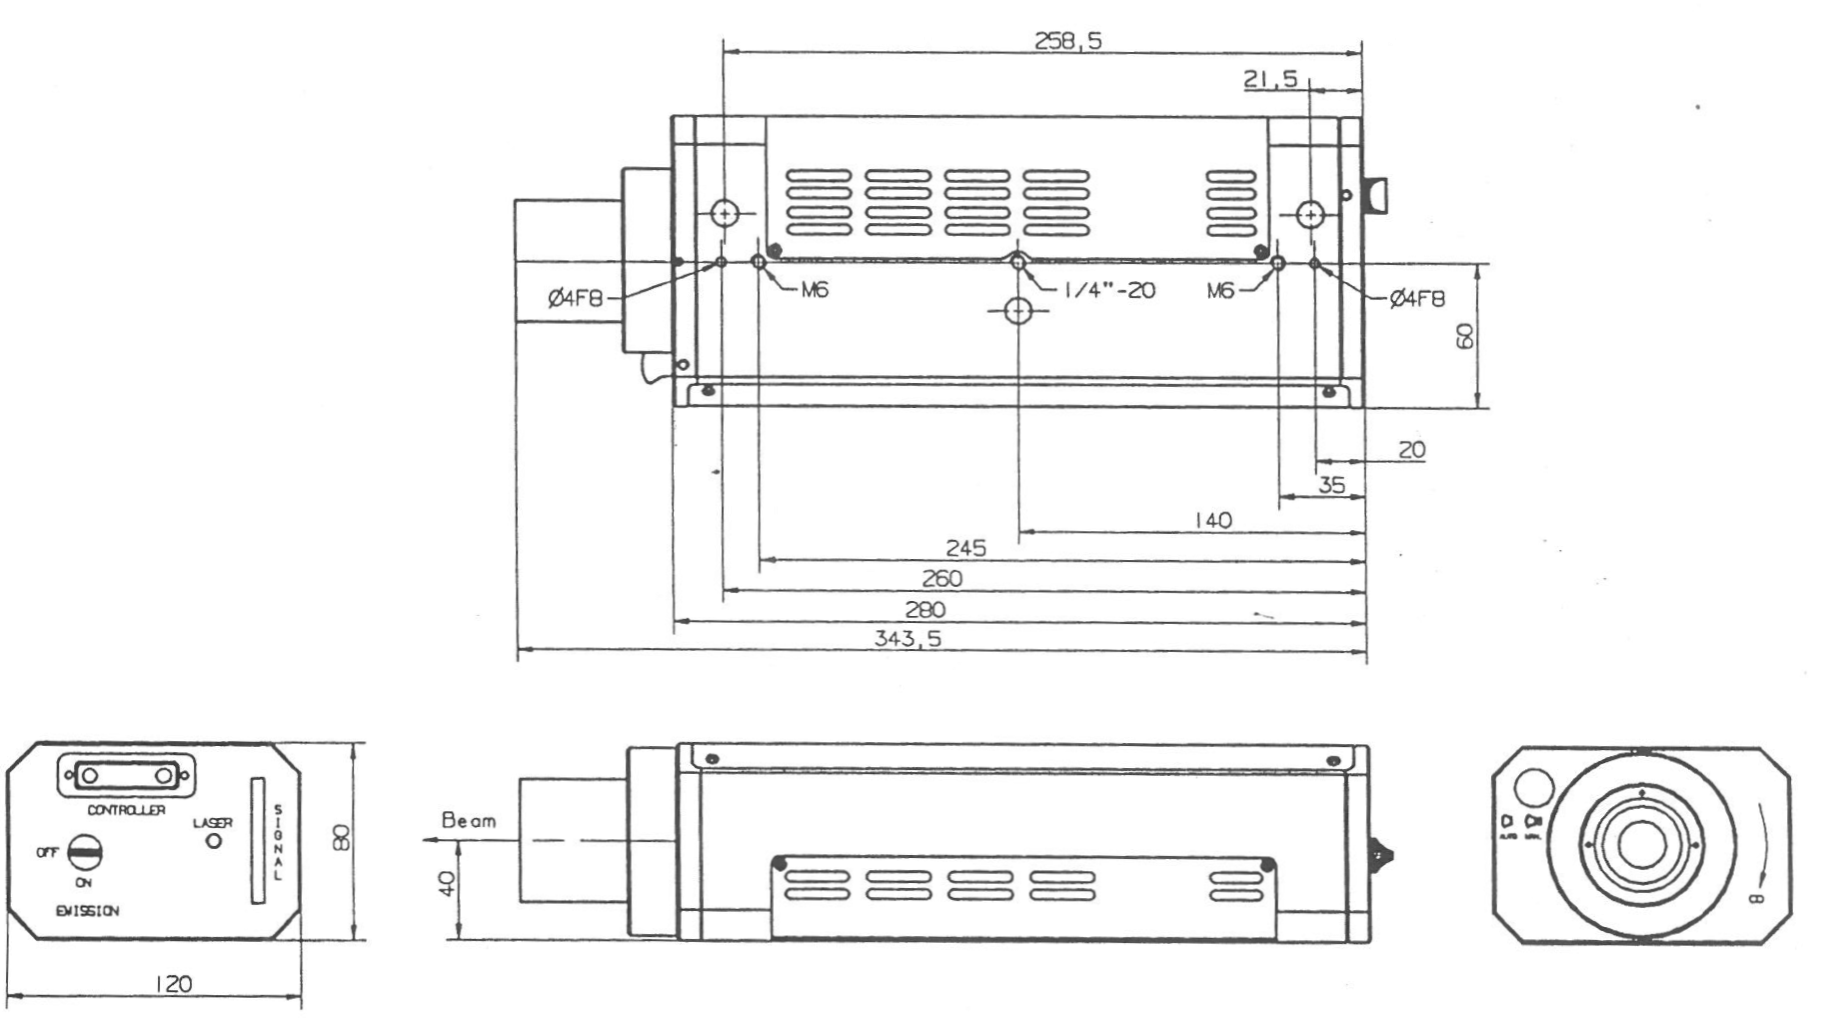
\includegraphics[width=0.8\textwidth]{img/wib_meas.png}
\caption{Wymiary głowicy OFV-353. Źródło: \cite{wib_docs} }
\label{img:wib_meas}
\end{figure}

Laboratorium Akustyki Technicznej (LAT) dysponuje wibrometrem wraz z głowicą OFV-353, i to pod tą głowicę projektowane będzie urządzenie. Można ją przybliżyć jako $3.5 kg$ prostopadłościan o wymiarach:
\vspace{-\topsep}
\begin{itemize}
    \item $280 mm$ wzdłuż osi $x$,
    \item $120 mm$ wzdłuż osi $y$,
    \item $80 mm$ wzdłuż osi $z$,
\end{itemize}
\vspace{-\topsep}
Zgodnie z rys. \ref{img:wib_meas}. \cite{wib_docs}
\subsection{Środek Masy}

Aby poprawnie poruszać wibrometrem, osie obrotów silników powinny obracać się w środku masy urządzenia. W przypadku systemów tak skomplikowanych jak wibrometr, najprostszą i najbardziej skuteczną metodą jest metoda doświadczalna. Próbując ustabilizować wibrometr w jednym punkcie, osiągnięto współrzędne środka masy. Jest to punkt odsunięty od środka geometrycznego o $\Delta_x = 1.5cm$. Gdzie oś $x$ to oś idąca wzdłuż dłuższego boku wibrometru razem z laserem wibrometru. W osi $y$ oraz $z$ środek masy jest zgodny ze środkiem geometrycznym. Biorąc poprawkę na gumowe podstawki wibrometru, środek masy jest odsunięty od ich spodu o $6cm$, co należy uwzględnić w modelu 3D.

\section{Jednostka napędowa}
\noindent Podczas projektowania stołu wzięto pod uwagę wiele różnych jednostek napędowych:
\subsection{Serwomechanizm modelarski}

\begin{figure}[h!] 
\centering 
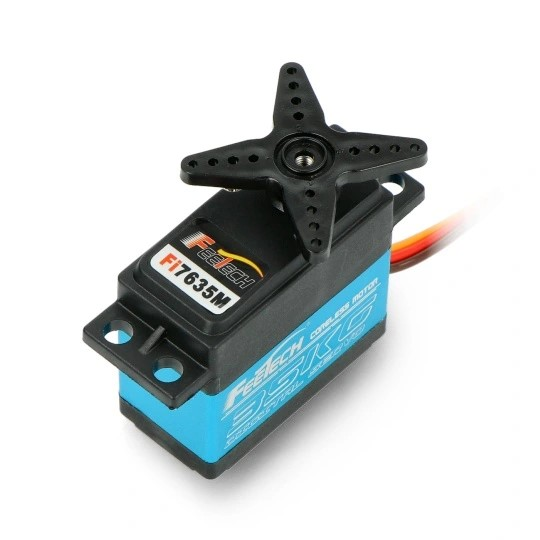
\includegraphics[width=0.5\textwidth]{img/feetech_servo.jpg}
\caption{Serwo Feetech FI7635M, przykładowe serwo modelarskie. Źródło: \cite{feetech_servo_docs}}
\label{img:feetech_servo}
\end{figure}

Pierwszym rozważanym typem jednostki napędowej był serwomechanizm modelarski (\textbf{standard servo}) (przykład na zdj. \ref{img:feetech_servo}). Serwa takie mają stosunkowo małe momenty obrotowe (sięgające do $35 kg \cdot cm$). Posiadają bardzo drobne, kruche przekładnie i z wielu wcześniejszych doświadczeń wynika, że nie są to trwałe rozwiązania. Problemem jest także zakres ruchu, który zwykle wynosi $+-180^{\circ}$. Serwo nie obróci się dalej niż pełne $360^{\circ}$, w środku znajduje się fizyczna blokada. (Wyjątkiem są serwa typu $360^{\circ}$, jednakże serwa te pozwalają na kontrolę prędkości obrotowej, nie pozycji.) Plusami serw modelarskich jest prostota obsługi. Pozycja jest proporcjonalna do wartości wypełnienia PWM sygnału podanego na pin sygnałowy serwomechanizmu, Dodatkowo posiadają one wbudowany enkoder absolutny, co powoduje że nawet po odcięciu zasilania serwo pamięta swoją pozycję. Jednakże ten typ jednostki napędowej został odrzucony, jako rozwiązanie nieadekwatne do tego zastosowania. Serwomechanizmy są zbyt małe, aby obsłużyć omawiany wibrometr. \cite{feetech_servo_docs}


\subsection{Silnik krokowy}
Kolejnym rozwiązaniem jakie sprawdziłoby się w takim zastosowaniu to silniki krokowe (\textbf{stepper motor}) (przykład na zdj. \ref{img:stepper}). Są one także bardzo proste do wysterowania. W zależności od podtypu silnika sterowanie różni się, ale zasada jest zawsze ta sama - należy jedynie podawać informacje o kolejnych krokach na sterownik, który obraca silnik o znany kąt, odpowiadający jednemu krokowi. Posiadają one jednak dużo niższe momenty obrotowe niż inne rozwiązania, a przekładnie zmniejszające prędkość a zwiększające moment są stosowane, ale raczej rzadko. A na pewno nie tak często jak z innymi jednostkami napędowymi. \cite{pololu_steppers}

\begin{figure}[h!] 
\centering 
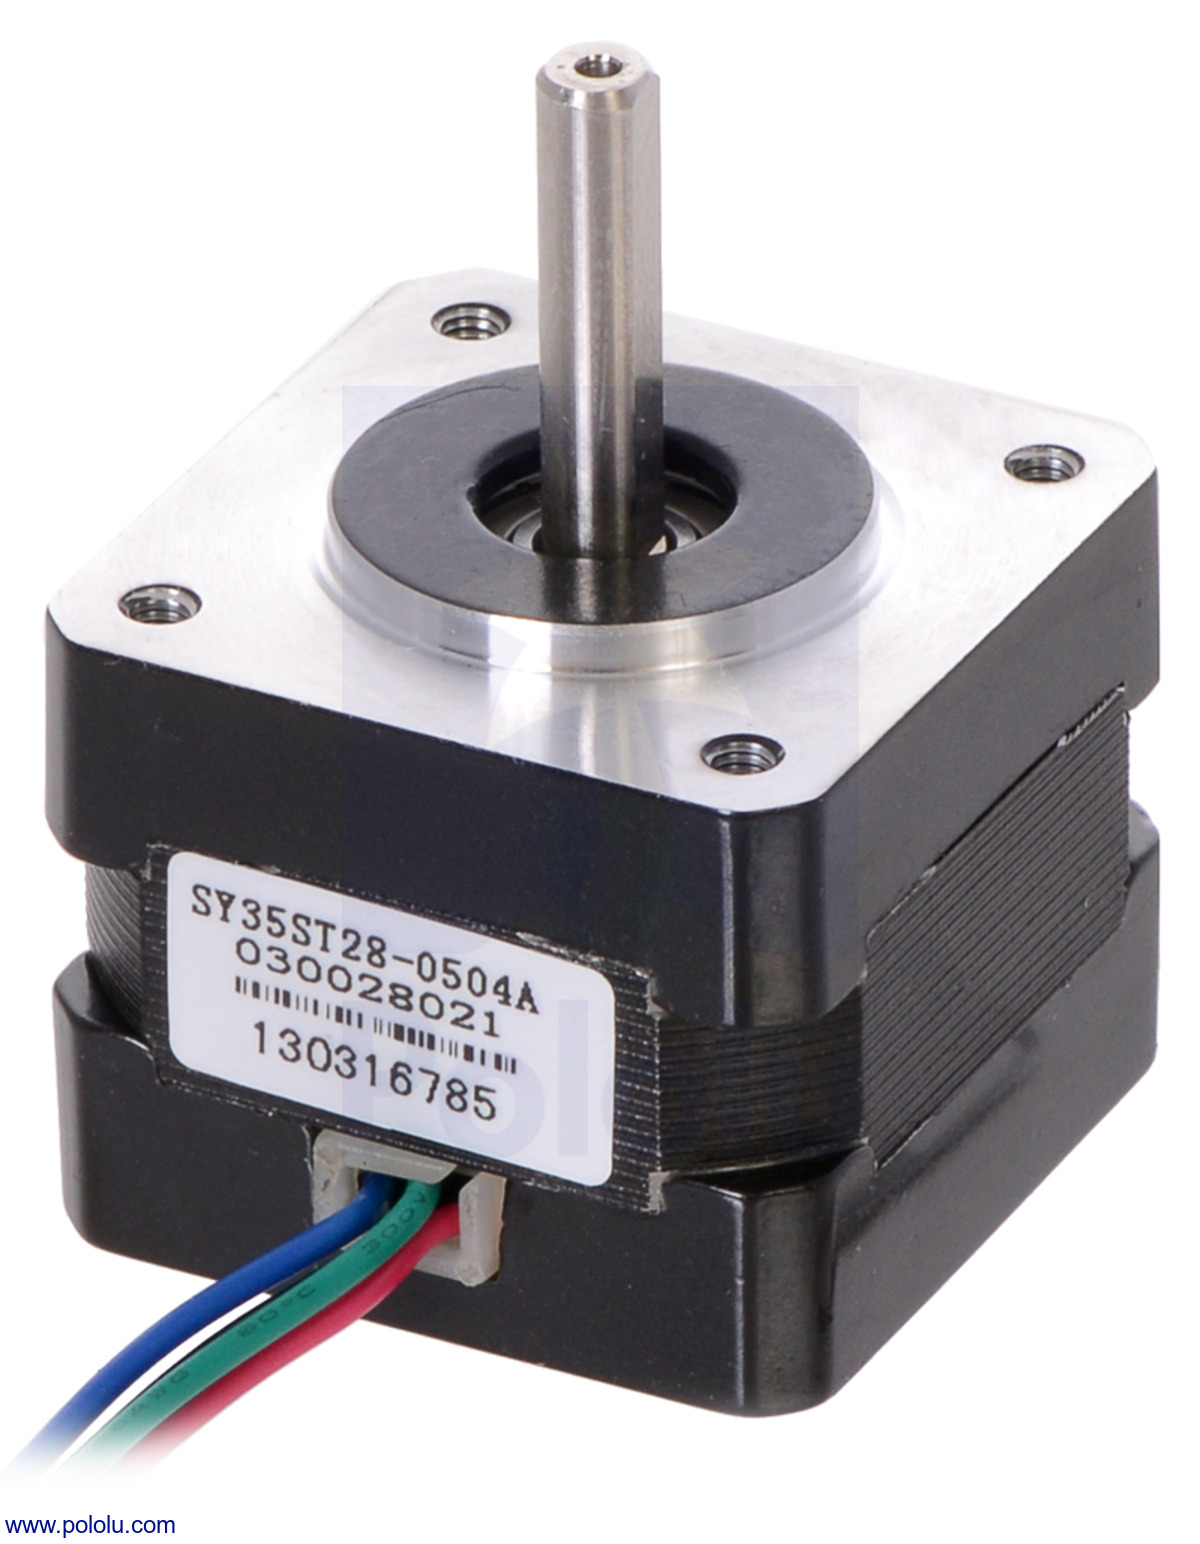
\includegraphics[width=0.4\textwidth]{img/stepper.jpg}
\caption{Silnik krokowy bipolarny, model Pololu 1208. Źródło: \cite{pololu_steppers}}
\label{img:stepper}
\end{figure}

Silniki mogą mieć różną precyzję, ale najczęściej spotykane są wartości rzędu od 100 do 400 kroków na obrót, co daje precyzję około $3.6^{\circ} - 0.9^{\circ}$, co może być za mało jak na ten projekt. \cite{motrioncontrol_stepper_guide} Precyzje potrafią sięgać aż do 1000 kroków na obrót przy droższych liniach silników, jednakże nie są one aż tak popularne jak wartości z rzędu setek kroków na obrót. \cite{pololu_stepper_forum}

Dodatkowo silniki krokowe mają duży pobór mocy, ponieważ nawet nieruchome pobierają prąd. Ostatecznie, przy silnikach krokowych zawsze istnieje ryzyko zgubienia kroku. Dlatego, jeżeli wymogiem jest znajomość pozycji z dużą dozą pewności, należałoby zastosować dodatkowy enkoder, który niezależnie sprawdzi czy nie nastąpiło zgubienie kroku.

Ostatecznie, silnik krokowy po dodaniu przekładni i dodatkowego enkodera byłby dobrym rozwiązaniem. Jednakże z powodu rozmiarów, i co za tym idzie bezwładności oraz wymaganego momentu, a także z powodu małej popularności gotowych rozwiązań łączących silnik krokowy, przekładnię oraz enkoder, pomysł zastosowania silnika krokowego został porzucony.

\subsection{Silnik szczotkowy prądu stałego}
\label{cha:brushed_dc_motor}
Ostatecznie najlepszym kandydatem okazał się być klasyczny silnik szczotkowy prądu stałego (\textbf{Brushed DC Motor}). Silniki te posiadają stosunkowo małe wymiary. Ponadto dołączenie przekładni daje bardzo duże momenty obrotowe, a zastosowanie enkodera daje realne sprzężenie zwrotne, mówiące o ruchu silnika. Poważnym utrudnieniem jest sposób ich sterowania. Nie są to silniki naturalnie przystosowane do kontroli pozycji. Pozycję należy odczytać z enkodera i na silnik podać sterowanie, odpowiadające prędkości obrotu silnika, które doprowadzi wał do pozycji docelowej. Jest to jednak utrudnienie, które jeżeli zostanie pokonane, da najlepsze rezultaty. Do projektu został wybrany silnik z linii Pololu 37D. Są to silniki z zamontowaną przekładnią, oraz w zależności od modelu, mają także enkoder. Jako że w projekcie tym priorytetem jest uciąg silnika, a nie prędkość kątowa wału, zdecydowano się na największą możliwą przekładnię, $150:1$. Dodatkowo wymogiem jest kontrola pozycji, dlatego wymagany jest wariant z enkoderem.

\begin{figure}[h!] 
\centering 
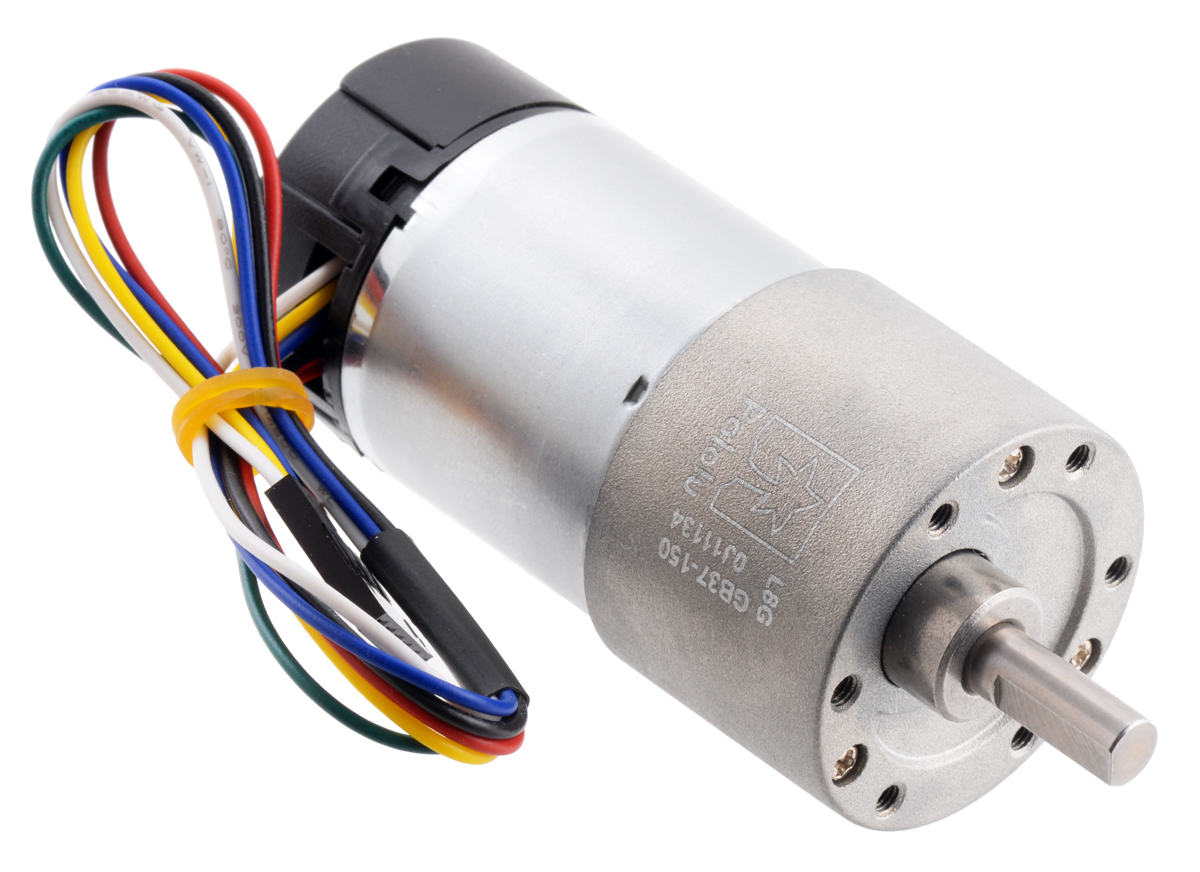
\includegraphics[width=0.4\textwidth]{img/pololu_2828.jpg}
\caption{Silnik szczotkowy prądu stałego Pololu 2828. Źródło: \cite{pololu_2828}}
\label{img:pololu2828}
\end{figure}

\noindent Po spełnieniu tych wszystkich kryteriów otrzymano silnik Pololu 2828 (przedstawionego na zdj \ref{img:pololu2828}), który \cite{pololu_2828}: 
\vspace{-\topsep}
\begin{itemize}
    \item Jest zasilany napięciem 12V
    \item Posiada prędkość obrotową bez obciążenia wynoszącą $67RPM$
    \item Moment obrotowy równy $49 kg \cdot cm$
    \item Bez obciążenia pobiera jedynie $200mA$
    \item Pod maksymalnym obciążeniem pobiera nawet do $5.5A$
    \item Posiada wbudowany enkoder o rozdzielczości $64CPR$, co po uwzględnieniu przekładni daje $9600CPR$.
\end{itemize}

\section{Modele 3D}
\subsection{Projekt}
Układ pozycjonujący wibrometr został zaprojektowany w układzie współrzędnych kątowych RPY, czyli kątów \textbf{Roll}, \textbf{Pitch}, \textbf{Yaw}, przedstawionych na rys. \ref{img:RPY}. Jak widać, oś obrót dookoła osi roll odpowiada obrotowi dookoła osi $x$, oś yaw odpowiada osi $z$ a oś pitch odpowiada osi $y$. 

\begin{figure}[h!] 
\centering 
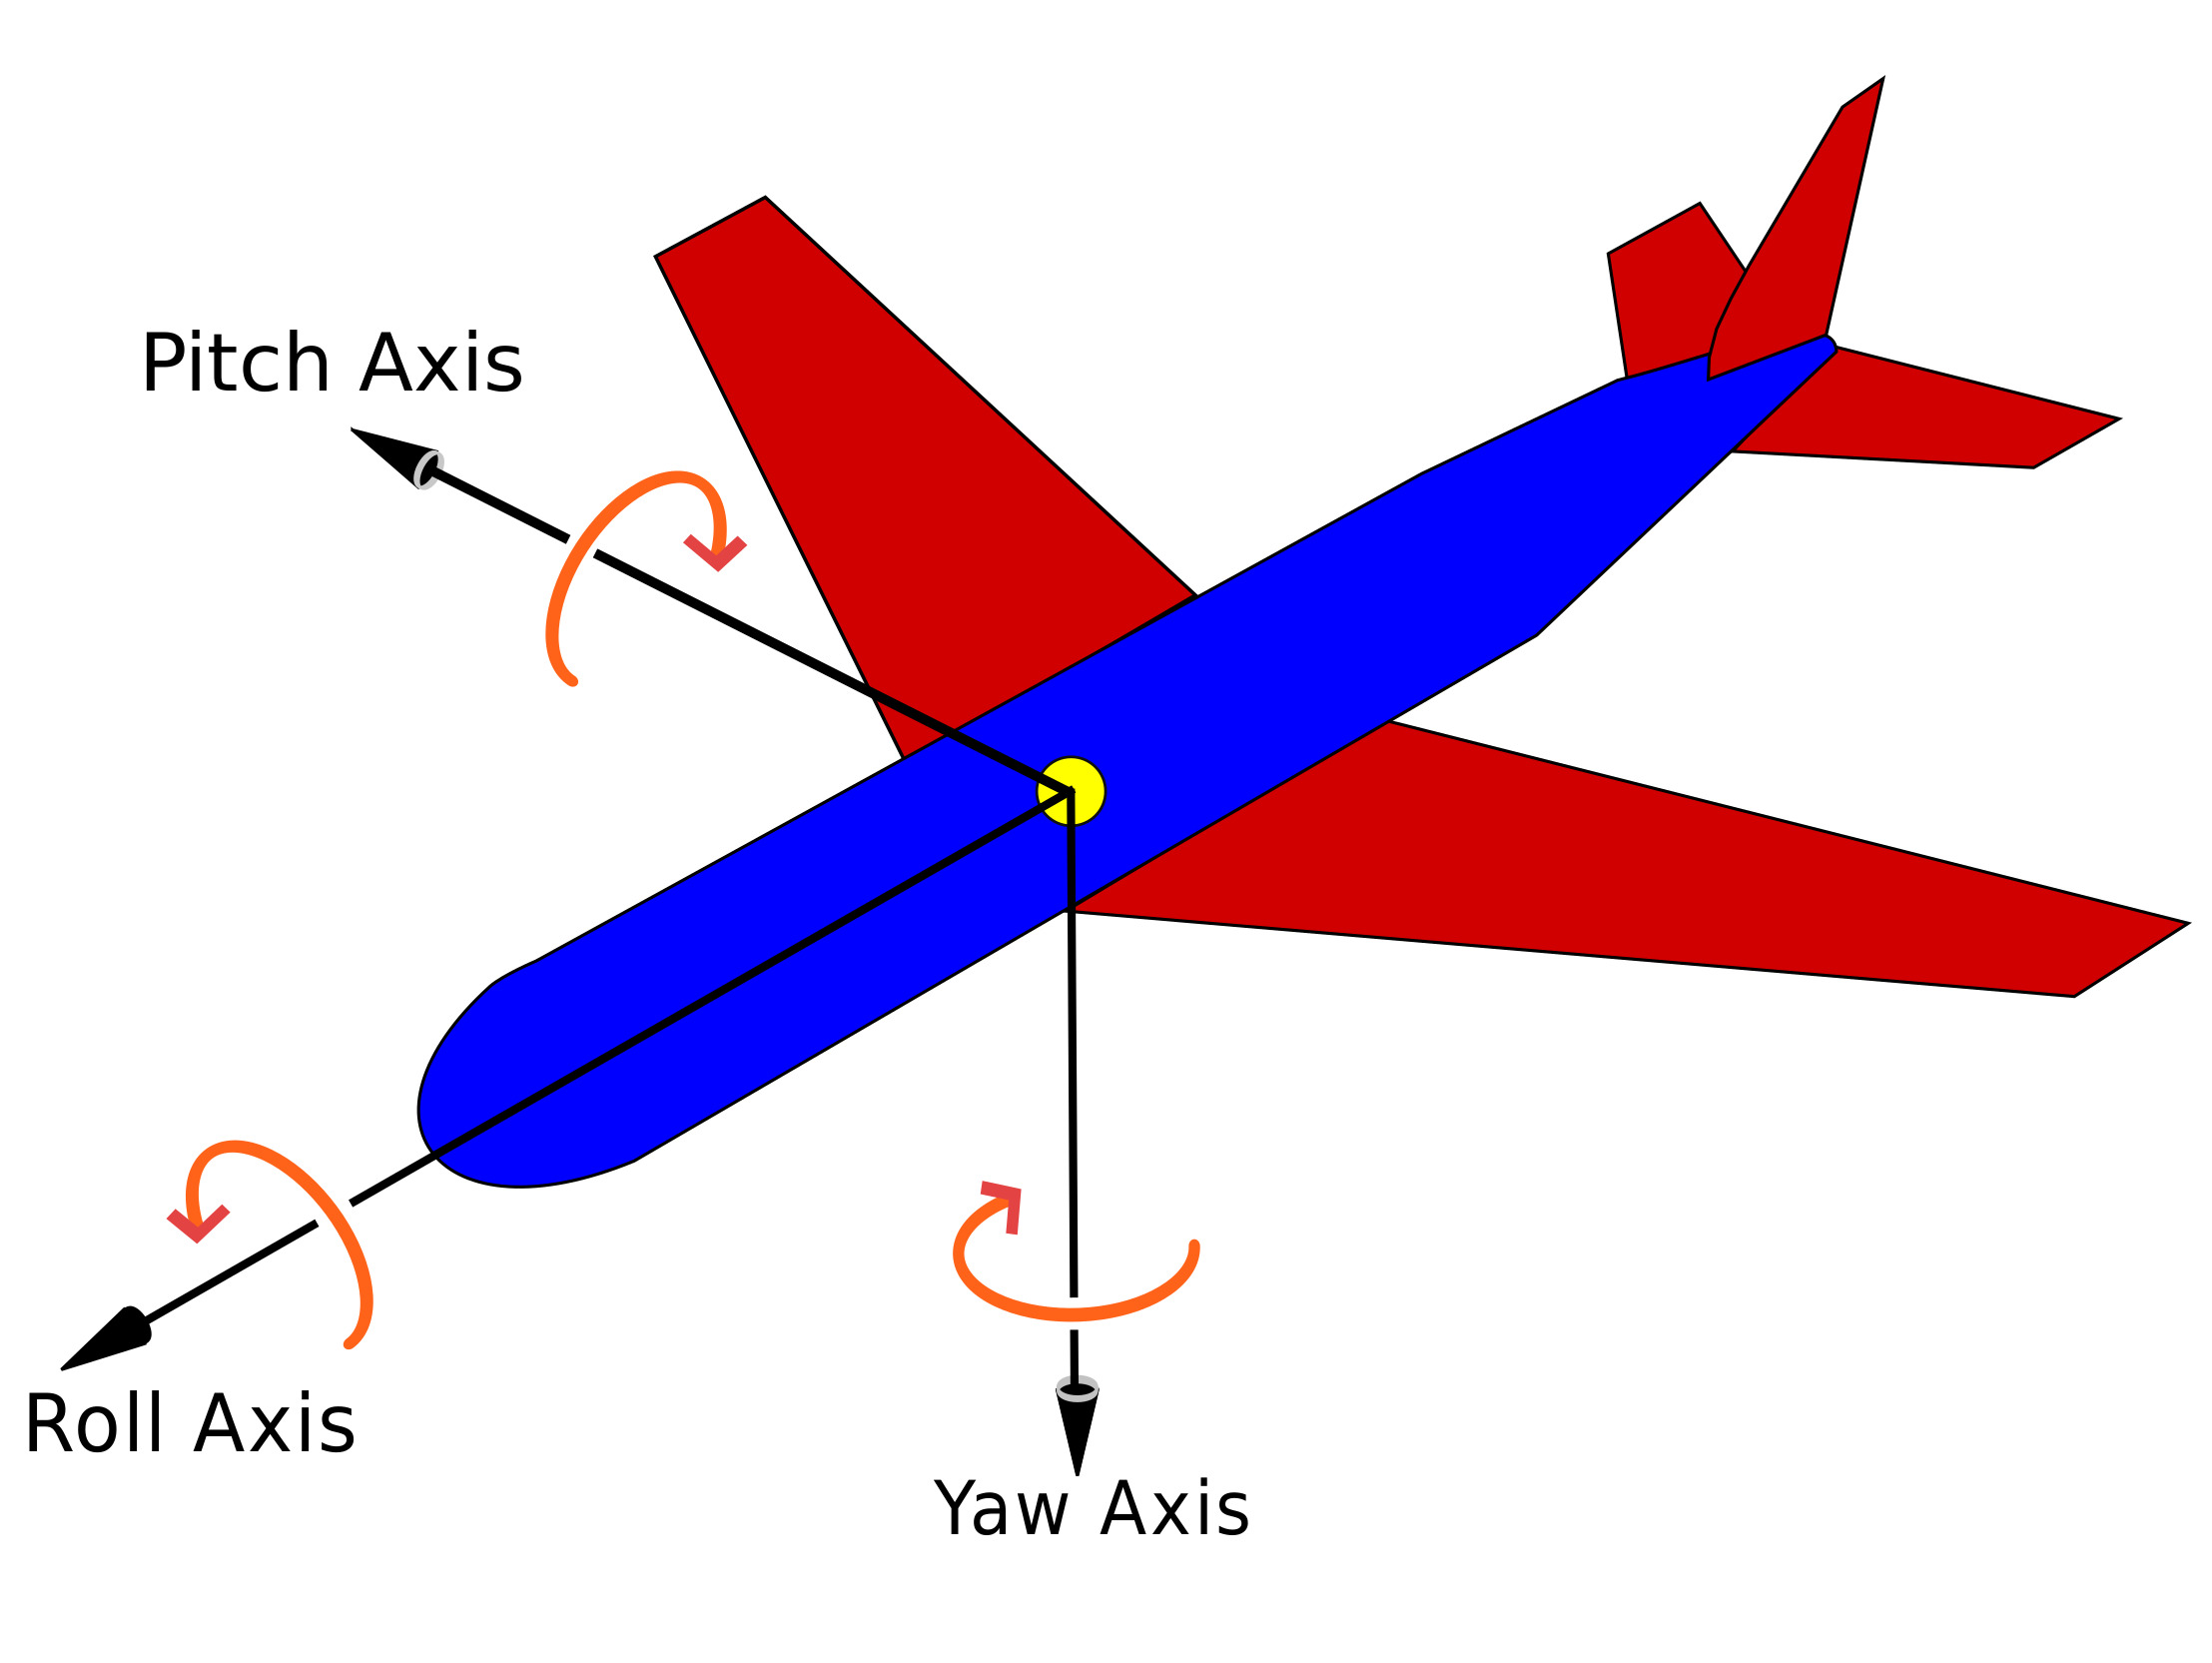
\includegraphics[width=0.6\textwidth]{img/RPY.jpg}
\caption{Osie RPY. Źródło: \cite{RPY_obrazek}}
\label{img:RPY}
\end{figure}

Celem pracy jest zaprojektowanie stołu, który obróci wibrometr dookoła osi yaw i pitch, natomiast laser wibrometru będzie poruszał się wzdłuż osi roll, która pozostaje nieruchoma.

\subsection{Wykonanie modeli}
\label{cha:3d_models_assembly}
Modele zostały wykonane w oprogramowaniu Autodesk Fusion 360. Jest to chmurowe oprogramowanie typu 3D CAD, pozwalająca na tworzenie modeli oraz całych złożeń. Zostało ono wybrane ze względu na opcje łatwego przechowywania modeli w chmurze, co pozwala na wygodną pracę na wielu komputerach na raz. \cite{Fusion_opis}

\begin{figure}[h!] 
\centering 
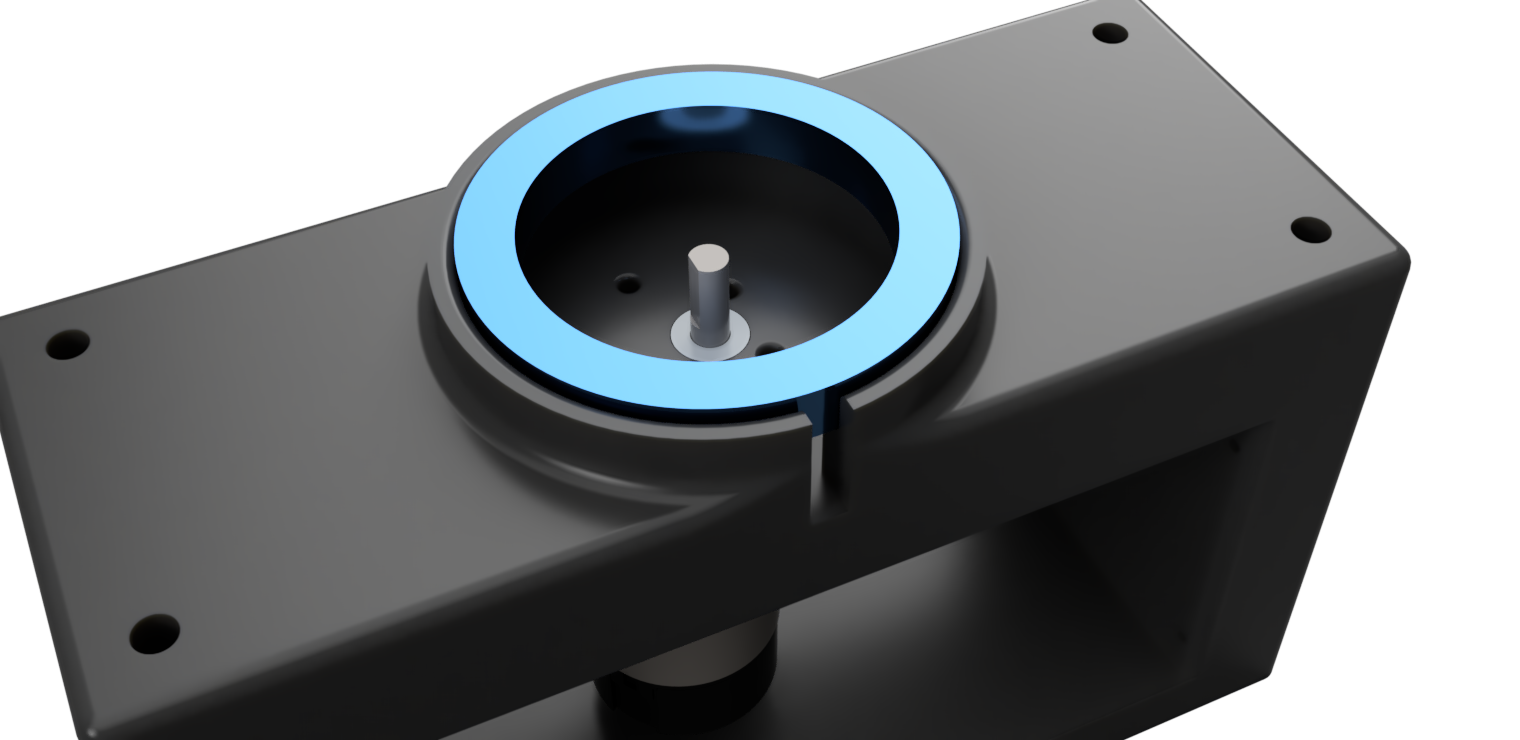
\includegraphics[width=0.6\textwidth]{img/Fusion1.png}
\caption{Złożenie części statycznej stołu oraz pierwszego silnika.}
\label{img:fusion_1}
\end{figure}

W pierwszej kolejności zostało opracowane połączenie między dolnym silnikiem, obracającym się dookoła osi yaw (z), a częścią stołu, która także ma się dookoła tej osi obracać. Na rys. \ref{img:fusion_1} można zauważyć, że statyczna część tego silnika jest przymocowana do statycznej części stołu. Na niej, dookoła wału, leży łożysko kulkowe o wymiarze $55x72x9mm$ (na \ref{img:fusion_1} zaznaczone niebieskim kolorem). Łożysko zostało zastosowane aby nie opierać masy wibrometru bezpośrednio na wale silnika. Kolejny krok, przedstawiony na rys. \ref{img:fusion_2}, prezentuje montaż wału do obrotowej części stołu. Wspomniana część jest przymocowana do wału poprzez gotowy hub montażowy Pololu 1083 (przedstawiony na rys \ref{img:pololu_hub}) oraz kilka dystansów, pozwalających odsunąć środkową, obrotową część stołu od wału silnika.

\begin{figure}[h!] 
\centering 
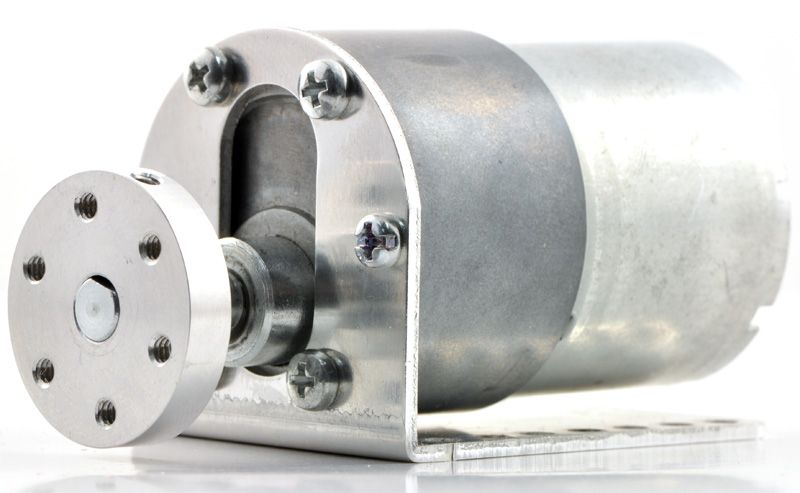
\includegraphics[width=0.3\textwidth]{img/pololu_hub.jpg}
\caption{Pololu Hub na wał 6mm (Pololu 1083). Źródło: \cite{Pololu_hub}}
\label{img:pololu_hub}
\end{figure}

Dodatkowo na obu rysunkach można zaobserwować, że środkowa, obrotowa część stołu jest umieszczona wewnątrz wspomnianego łożyska, leży na wewnętrznym jego pierścieniu. Natomiast dolna, statyczna część stołu znajduje się na zewnątrz łożyska. Łożysko spoczywa swoim zewnętrznym pierścieniem na statycznej części stołu. Dodatkowo rys. \ref{img:fusion_1} przedstawia otwór, pozwalający przykręcić wspomniany wcześniej hub do wału silnika.


\begin{figure}[h!] 
\centering 
\begin{subfigure}{.4\textwidth}
  \centering
  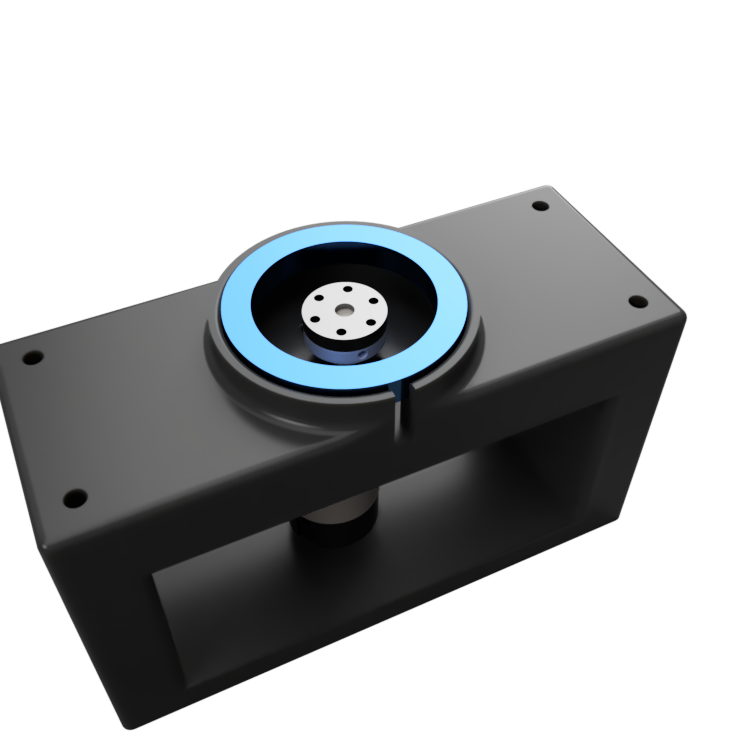
\includegraphics[width=\textwidth]{img/Fusion2a.png}
\end{subfigure}%
\begin{subfigure}{.4\textwidth}
  \centering
  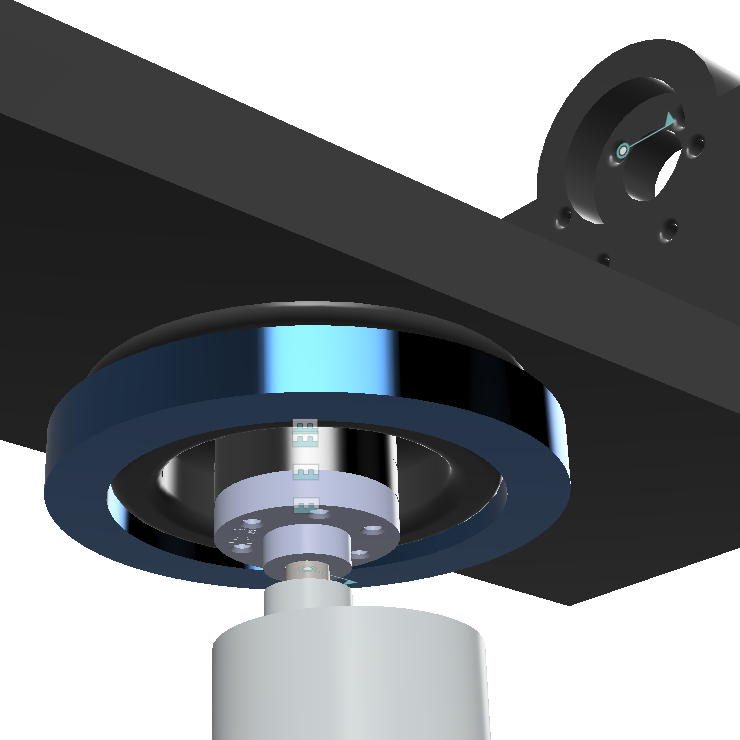
\includegraphics[width=\textwidth]{img/Fusion2b.png}
\end{subfigure}
\caption{Montaż wału silnika do środkowej części obrotowej.}
\label{img:fusion_2}
\end{figure}

Kolejnym krokiem było przymocowanie drugiego silnika do środkowej, obrotowej części, tak aby nadać konstrukcji drugą oś swobody. Montaż samego silnika jest przedstawiony na rys. \ref{img:fusion_3a}. Na wał silnika także został zamontowany hub mocujący, który, aby odciążyć sam wał, został wsunięty w łożysko, które w tym miejscu ma wymiary $12x28x8mm$ (Zaznaczone na rys. \ref{img:fusion_3b} kolorem czerwonym). Do huba przymocowana jest część tzw. Holder, która ma podtrzymywać wibrometr. Ma ona już obie osie swobody, potrafi się obracać dookoła osi yaw dzięki pierwszemu silnikowi, jak i dookoła osi pitch dzięki drugiemu silnikowi. Symetrycznie, naprzeciwko silnika drugiego, także znajduje się otwór pod łożysko. Jednakże w tym miejscu nie montujemy silnika, a zamiast niego Holder podobny do tego montowanego do huba. Opisywany, drugi Holder, zamiast otworów montażowych do huba, posiada własny wał wkładany w łożysko. Montaż tych dwóch części widoczny jest na rys. \ref{img:fusion_4}.

\begin{figure}[h!] 
\centering 
\begin{subfigure}{.6\textwidth}
\centering 
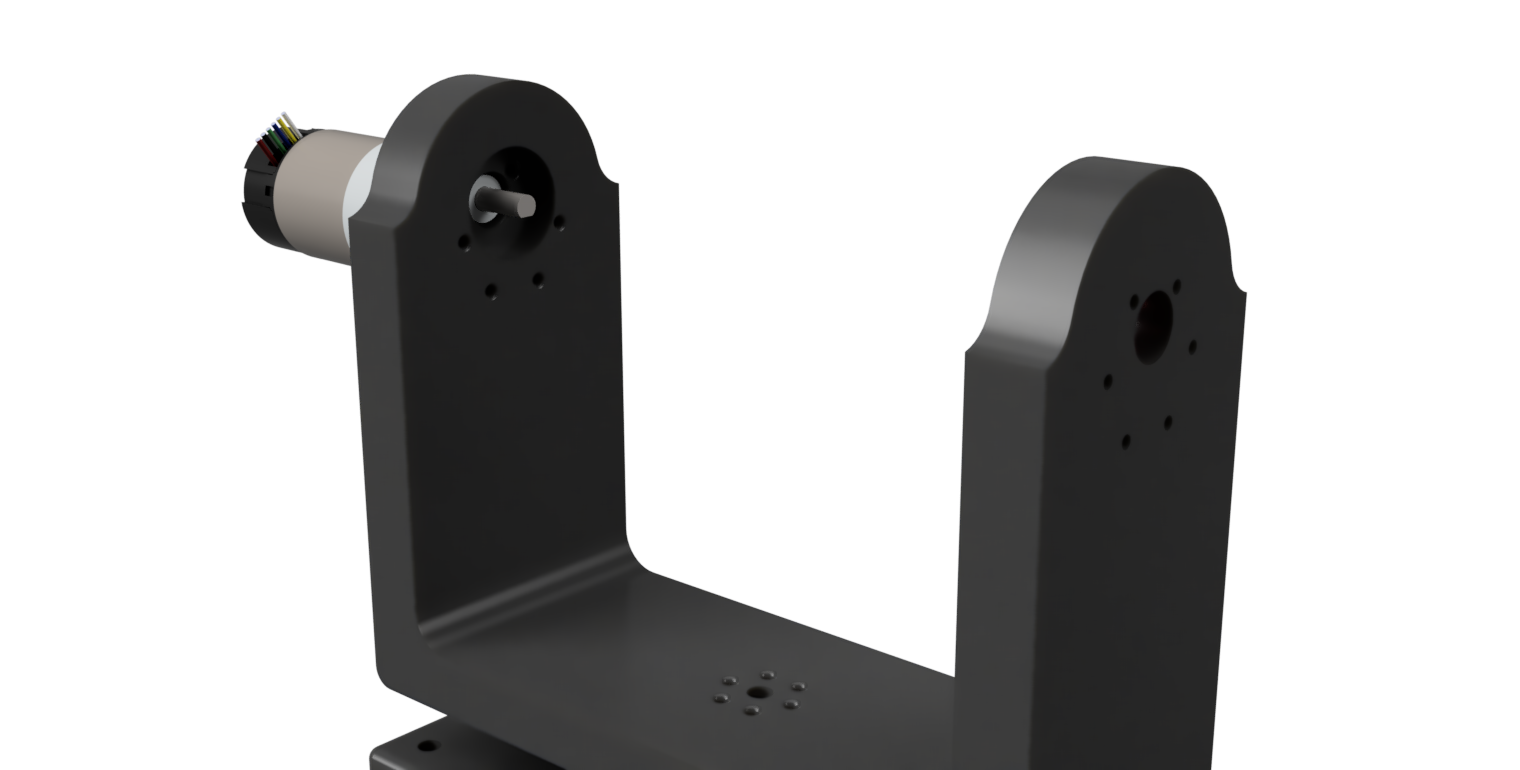
\includegraphics[width=\textwidth]{img/Fusion3a.png}
\caption{Montaż drugiego silnika do części ruchomej obrotowej}
\label{img:fusion_3a}
\end{subfigure}%
\begin{subfigure}{.4\textwidth}
\centering 
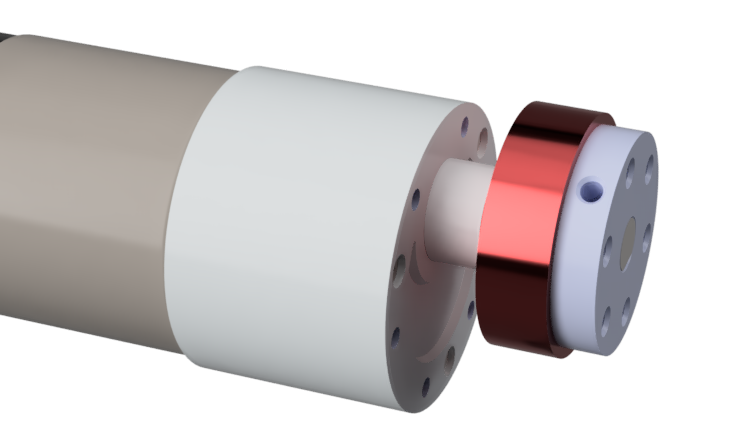
\includegraphics[width=\textwidth]{img/Fusion3b.png}
\caption{Montaż łożyska oraz hub-a montażowego do drugiego silnika}
\label{img:fusion_3b}
\end{subfigure}
\label{img:fusion_3}
\caption{Montaż drugiego silnika.}
\end{figure}

\begin{figure}[h!] 
\centering 
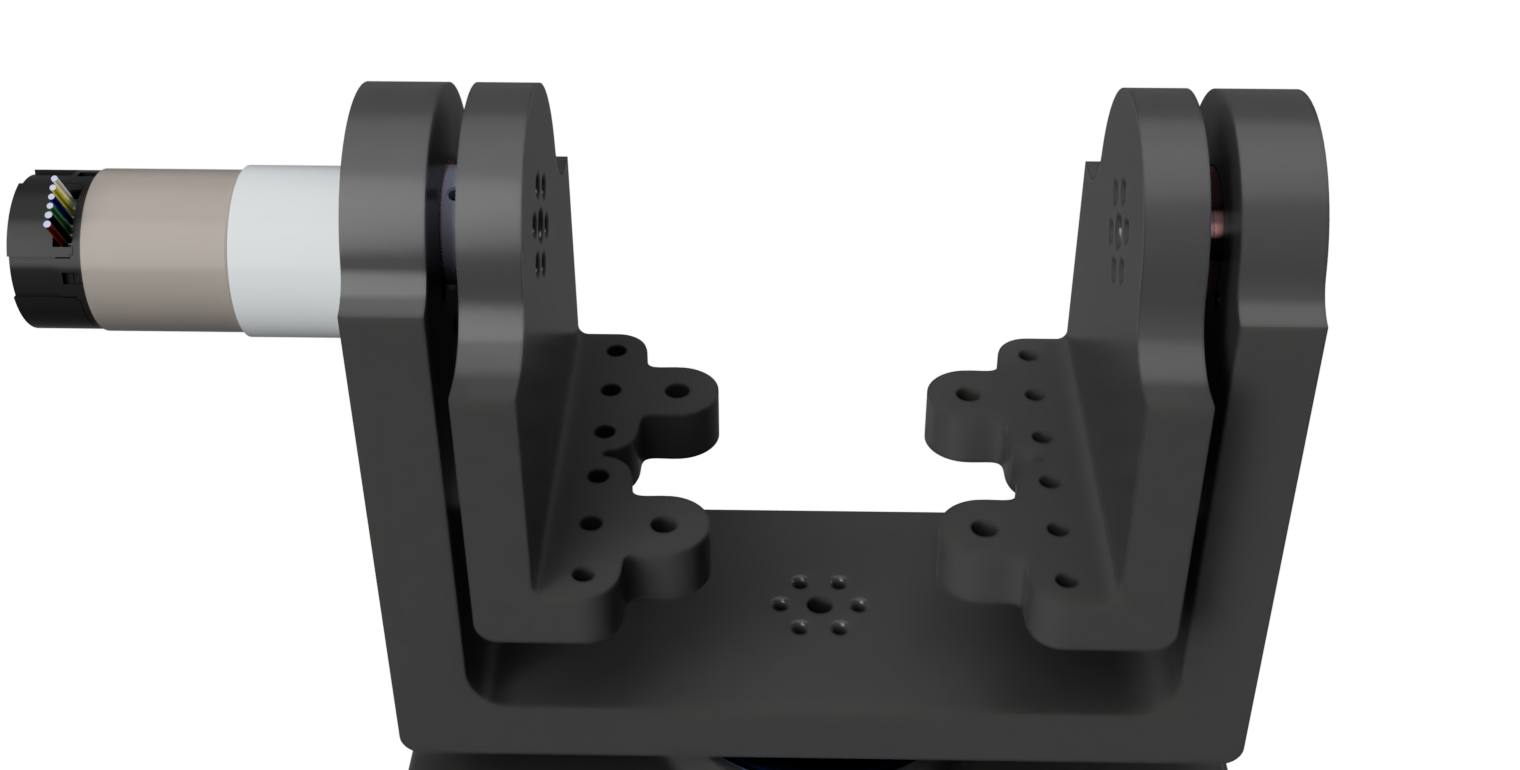
\includegraphics[width=0.7\textwidth]{img/Fusion4.png}
\caption{Montaż obu holderów do reszty modelu.}
\label{img:fusion_4}
\end{figure}

Oba holdery podtrzymują płytę, do której przykręcany jest wibrometr. Obrazuje to rys. \ref{img:fusion_5}, który przedstawia całość stołu pozycjonującego wibrometr dookoła osi yaw oraz pitch w układzie współrzędnych RPY.

\begin{figure}[h!] 
\centering 
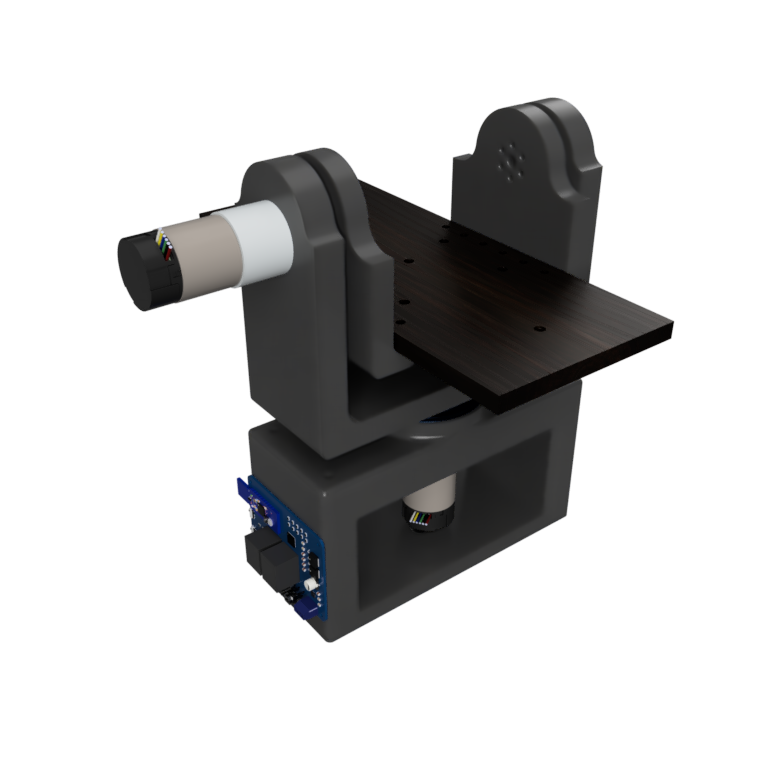
\includegraphics[width=1\textwidth]{img/Fusion5.png}
\caption{Model całej złożonej konstrukcji.}
\label{img:fusion_5}
\end{figure}
